\documentclass[12pt]{article}

\usepackage[english]{babel}
\usepackage[utf8]{inputenc}
\usepackage[T1]{fontenc}
\usepackage{graphicx}
\usepackage{caption}
\usepackage{anysize}
\usepackage{amsmath}

\usepackage{hyperref}
\hypersetup{
	pdftitle = {IS - TP1}
	,pdfauthor = {João Ferreira \& João Silva\\ Departamento de Engenharia Informática\\ Universidade De Coimbra\\ \texttt{jpbat@student.dei.uc.pt | jfmsilva@student.dei.uc.pt}}
	,pdfborder = {0 0 0}
}

\title{Enterprise Application Integration \\ Practical Assignment 2}
\author{
		João Ferreira \& João Silva\\
		Departamento de Engenharia Informática\\
		Universidade de Coimbra\\
		\texttt{jpbat@student.dei.uc.pt | jfmsilva@student.dei.uc.pt}\\
		\texttt{2009113274 | 2008111448}
		}
\date{November 2013}

\begin{document}
\maketitle
\clearpage

\tableofcontents

\setlength{\parindent}{1cm}
\setlength{\parskip}{0.3cm}

\clearpage
\section{Introduction}
\indent \indent In this practical assignment it was requested that we reused the first one (just the crawler) to populate a database using JPA.

As the both of us had made the first assignment separated, our first step was to decide wich one of the crawlers to use.

Once the database was populated we used that data to later build a web site, in wich the user could log in and browse through the movies and sort them alfabetically or filter them either by score (bigger then, smaller then, or between an interval).

Besides that the user could also set his favorite list wich alowed him to receive email updates, each time a movie that belonged to at least one of his favorite catogories was added.

We'll now briefly explain some decisions that were taken and how we solved some issues that appeard along the way.
\clearpage

\section{Data Model}
\indent \indent We used the classes that were generated on the first assignment, and we added some anotations, so that the tables were automaticly generated.

So that we can understand better we attach an ER model from our database.

\begin{figure}[h!]
	\centering
	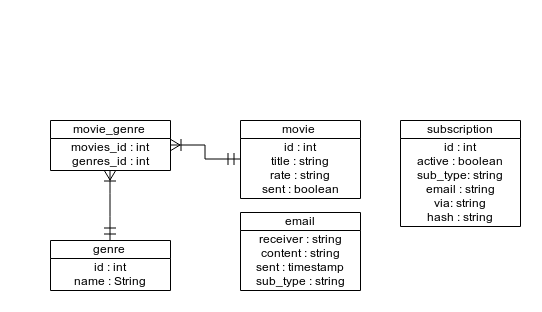
\includegraphics[width=\textwidth]{er.png}
	\caption{ER Model.}
\end{figure}

As we can see we have some weak entities that make the connection between our main entities (Acount, Movie, Genre). We decided that that was the best decision to take, once the other option was to put the full string in each one of the entities. With that option we can make any conection between the entities in a much simpler and faster way.

For instance, instead of searching the substring ``Drama'' in each of the Movies genre string, we can just request to the database all the movies id that had that connection in the Genre\_Movie table.

Since we needed the foreign relations from the movies and the users in most cases, we decided not to use the lazy loading from the database.
\clearpage

\section{Enterprise JavaBeans}
\indent \indent While creating the business logic layer, we implemented the CRUD (Create, Read, Update and Delete) class. This class contains all the primary functionalities and initialisations used by the Beans.
We created the following Beans:
\begin{description}
	\item [AccountService]: Statefull Bean to store the User information on log.

	\item [AccountManagerService]: Stateless Bean used to Search users in the Database.

	\item [EmailService]: Singleton Bean used to create an EmailDipatcher when the server starts and to give access to the mail queue.

	\item [MovieManagerService]: Message Driven Bean responsible for receiving new movie lists from the topic and sending the new Movies to the Database and to ask the Email dispatcher to send Emails to the users reporting new movies.

	\item [DirectorService]: Stateless Bean Used to perform basic operations related to Actors.

	\item [GenreService]: Stateless Bean Used to perform basic operations related to Genres.

	\item [MovieService]: Stateless Bean Used to perform basic operations related to Movie. We also added custom query’s to access the database like search by genre and filter by score.
\end{description}
All the queries to the database are created using the CriteriaBuilder to prevent SQL injection.
\clearpage

\section{Navigation}
\indent \indent To navigate through the website the user can access to three diferent pages. The mapping of the pages is made with Java Servlets and the pages are built with JSP.

In the top of the page, there is always either the information about the logged in user or a login form.

\subsection{Login}
\indent \indent In this page the user can either register filling a small form with important information.
Besides that an already registred user can login into the application, by filling the form available in the top of the page.

\subsection{Index}
\indent \indent In this page the user can filter the movies that are showed, order them in alfabetically, access to his personal page by clicking his name, and logout by hovering the mouse over his picture.

The filtering and sorting are accessed by clicking on the button available on the top of the page. A modal is showed in wich the user can select the desired option.

\subsection{Me}
\indent \indent In this page the user can edit his favorites and see the movie with the best score that belongs to one of his favorite categories.

\subsection{Protections}
\indent \indent Besides what was already said about the SQL Injection, we also protected the aplication against either access to unauthorized pages and scripting injection in the forms.
\clearpage

\section{Division of Work}
\indent \indent The work was, in what appeard to us, equally divided.
\begin{description}
	\item [João Ferreira] navigation, business model. (40h)
	\item [João Silva] entities, business model. (40h)
\end{description}
\clearpage

\section{Conclusion}
\indent \indent With this project we reforced idea that the abstraction of comunication is really important.

We also understood the importance of the usage of statefull and stateless beans, as well as the importance of keeping the implementation simple and as abstract from what we are trying to do as possible.

With this we consider that the execution of this assignment was a success, for wich the both of us learned some important aspects of the importance of using JPA to communicate with a database, along other things.
\clearpage

\begin{thebibliography}{9}
\bibitem{eai blog}
	\href{http://eai-course.blogspot.pt/}{Professor Filipe Araújo blog}.

\bibitem{jQuery}
	\href{http://jquery.com/}{jQuery website}.

\bibitem{Twitter Bootstrap}
	\href{http://getbootstrap.com/}{Twitter's Bootstrap website}.

\bibitem{W3Schools}
	\href{http://www.w3schools.com/}{W3Schools website}.
	
\bibitem{jboss community}
	\href{https://community.jboss.org/}{JBoss community}.
\end{thebibliography}
\end{document}